\chapterimage{Pictures/Ausberto/4_projeto.png} % Table of contents heading image

\begin{comment}
    Prof. Dr. Ausberto S. Castro Vera
    UENF - CCT - LCMAT - Curso de Ciência da Computação
    Campos, RJ,  2022
    Disciplina: Análise e Projeto de Sistemas
    Aluno: João Vítor Fernandes Dias
\end{comment}

\chapter{Projeto do Sistema}
    Neste capítulo, Falaremos sobre o projeto do sistema.
    
    \section{Estratégia do Projeto}
        Este projeto tem como estratégia o \textbf{desenvolvimento personalizado} pois visa atender às necessidades específicas da instituição que efetivar este projeto.
        
    % \section{Refinamento dos Diagramas DFD e E-R}
    %     Já tendo visto alguns diagramas de Fluxo de dados e de Entidade e Relacionamento, temos agora, representado pelas imagens A e B, esses diagramas, agora refinados.
    
    \section{Arquitetura do Sistema - Estilos}
        Temos abaixo alguns estilos de arquiteturas de sistema que serão ilustradas através de figuras.
        
        \subsection{Arquitetura do Sistema}
            Na arquitetura do sistema buscará seguir os padrões da Engenharia de Software. Principalmente ao que se trata do esperado envolvendo o design e construção. Utilizando de princípios como o de Desenvolvimento com testes e reuso de código.
        
        \subsection{Arquitetura do Hardware}
            Na arquitetura de hardware representada pela Figura \ref{Diagrama_de_Hardware}, vemos que o sistema terá diversas áreas de abrangência dentro da universidade, sendo eles os seus centros que permitirão acesso a diversos computadores em rede, e também acesso à impressora, sendo possível até mesmo o acesso à rede sem fio. O sistema precisará passar por um roteador que terá proteção de Firewall, e um outro roteador permitirá acesso aos bancos de dados.
            
            \begin{figure}[htbp]\centering
                \caption{Diagrama de arquitetura de Hardware}
                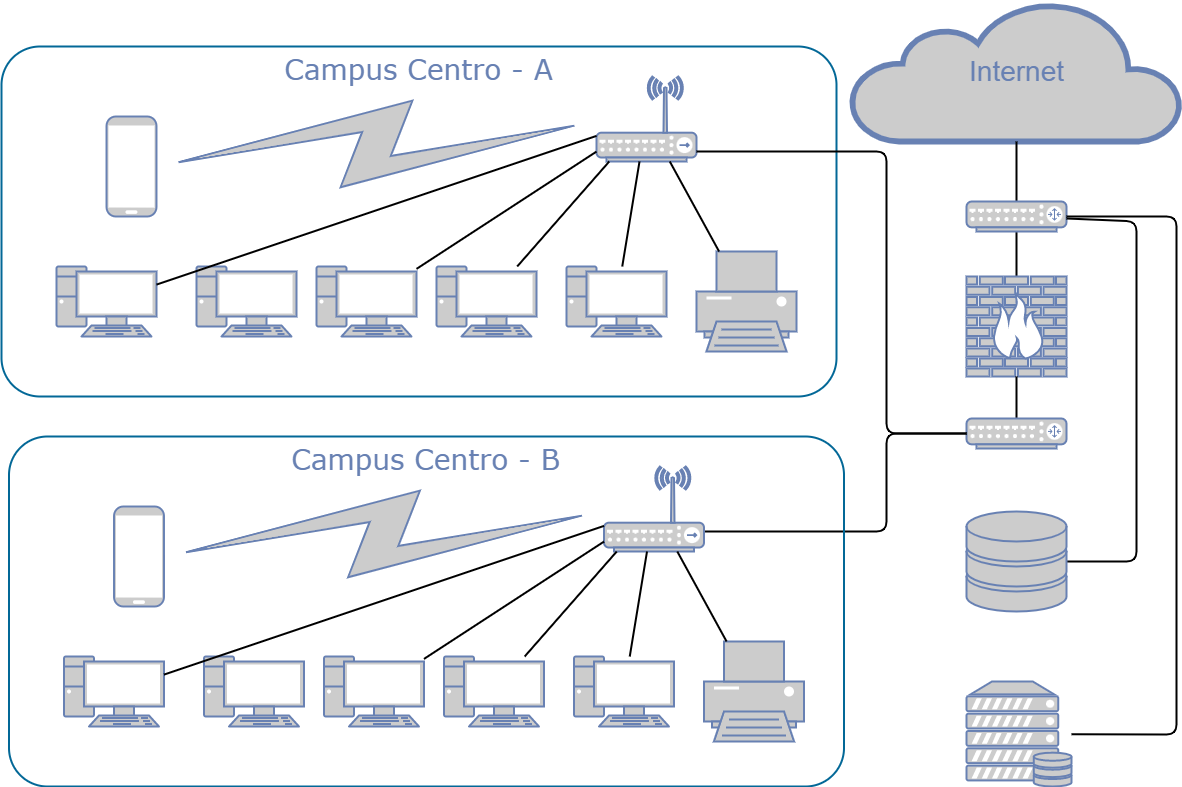
\includegraphics[angle=0,scale=0.3]{Pictures/JV/Arquitetura de Hardware.png}
                \label{Diagrama_de_Hardware}
            \end{figure}    % IMAGEM CRONOGRAMA DE ATIVIDADES
        
        % \subsection{Arquitetura de Software}
        %     Na arquitetura de software representada pela Figura XXX, vemos que...
    
    % \section{Projeto de Interface}
    %     Como projeto de interface, podemos ver o seguinte: